\documentclass[hyperref={pdfpagelabels=false}]{beamer}
\usepackage{lmodern}
\usepackage[T1]{fontenc}
\usepackage[utf8]{inputenc}
\usepackage{textpos}
\usepackage{hyperref}
\usepackage{listings}
\usepackage{graphicx}
\usepackage{amssymb}
\usepackage{minted}
\usepackage[minted]{tcolorbox}
\usepackage{xcolor}
\usepackage{textcomp}
\usepackage{pgffor}
\usepackage{todonotes}
\usepackage{tikz}
\usepackage{xifthen}

% Custom commands
\let\todox\todo
\renewcommand\todo[1]{\todox[inline]{#1}}

\newcommand{\textapprox}{\raisebox{0.5ex}{\texttildelow}}
\newcommand{\animation}[3][1]{%
	\foreach \n [count=\xi] in {1,...,#3}{%
		\includegraphics<\xi>[width=#1\textwidth]{#2\n.pdf}
	}
}

% TikZ setup
\tikzset{
  align at top/.style={baseline=(current bounding box.north)},
  invisible/.style={opacity=0},
  visible on/.style={alt={#1{}{invisible}}},
  alt/.code args={<#1>#2#3}{%
    \alt<#1>{\pgfkeysalso{#2}}{\pgfkeysalso{#3}} % \pgfkeysalso doesn't change the path
  },
}

\newcommand{\relc}[5]{
\node [anchor=west, visible on=<1->] at (#1.east) (#2) {#3};
\ifthenelse{\isempty{#4}}%
    {}
    {\node [anchor=west,fill=#5, visible on=<#4>] at (#1.east) (#2) {#3};}
}
\newcommand{\relcf}[4]{
\node [visible on=<1->] (#1) {#2};
\ifthenelse{\isempty{#3}}%
    {}
    {\node [fill=#4, visible on=<#3>] (#1) {#2};}
}
\newcommand{\relcbg}[4]{
\node [anchor=west,fill=#4] at (#1.east) (#2) {#3};
}
\newcommand{\relcbgf}[3]{
\node [anchor=west,fill=#3] (#1) {#2};
}

\newcommand{\fphalf}[1]{
\def\names{#1}
\begin{tikzpicture}[>=latex,font=\sffamily,every node/.style={minimum width=0.5cm,minimum height=0.6cm,inner sep=1pt,outer sep=0pt,draw=black,text=white,semithick}]
    \relcbgf{a1}{\StrMid{#1}{1}{1}}{purple}
    \foreach \n in {2,...,6}
    {
       	\pgfmathtruncatemacro\ystart{\n-1}
       	\relcbg{a\ystart}{a\n}{\StrMid{#1}{\n}{\n}}{darkgreen}	
    }
    \foreach \n in {7,...,16}
    {
       	\pgfmathtruncatemacro\ystart{\n-1}
       	\relcbg{a\ystart}{a\n}{\StrMid{#1}{\n}{\n}}{lightblue}
    }
\end{tikzpicture}
}

\usetikzlibrary{matrix,positioning,arrows.meta,arrows}

\definecolor{darkgreen}{rgb}{0.137, 0.5, 0.441}
\definecolor{lightblue}{rgb}{0.36, 0.54, 0.66}

% Beamer setup
\usetheme{metropolis}
\setbeamertemplate{footline}{%
	\hbox{%
		\begin{beamercolorbox}[wd=.7\paperwidth,ht=0cm,left]{author in head/foot}%
			\hspace*{2ex}\insertsection{}
		\end{beamercolorbox}%
		\begin{beamercolorbox}[wd=.3\paperwidth,ht=0cm,right]{date in head/foot}%
			\insertframenumber{} / \inserttotalframenumber\hspace*{2ex} 
	\end{beamercolorbox}}%
}

\setbeamertemplate{footnote}{
	\raisebox{0.1cm}{\insertfootnotemark \insertfootnotetext}
}

\setbeamertemplate{navigation symbols}{}

\graphicspath{{./img/}}

\setminted[cpp]{tabsize=4}\setminted[r]{}

\title{Going down the CPU microarchitecture\\rabbit hole}
\subtitle{Ramifications of CPU \& memory design}
\author{Jakub Beránek\\\href{mailto:jakub.beranek@vsb.cz}{\beamergotobutton{jakub.beranek@vsb.cz}}}
\date{16. 1. 2019}

\begin{document}

\begin{frame}
	\titlepage
\end{frame}

\begin{frame}{HPC}
    \begin{center}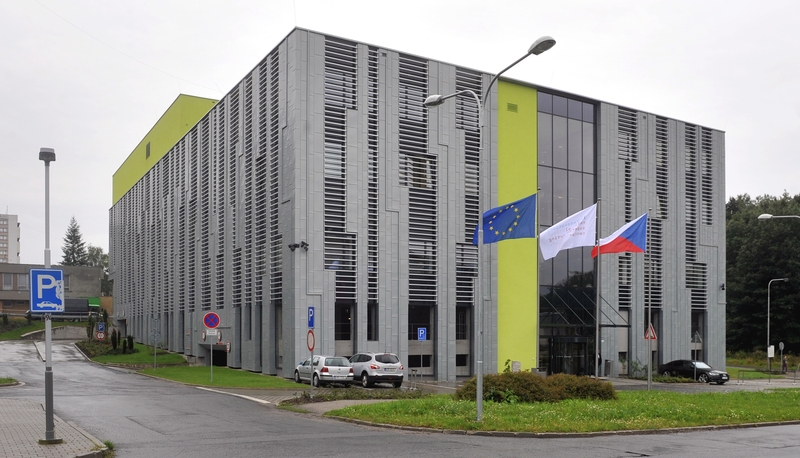
\includegraphics[width=0.5\textwidth]{it4i}\end{center}
    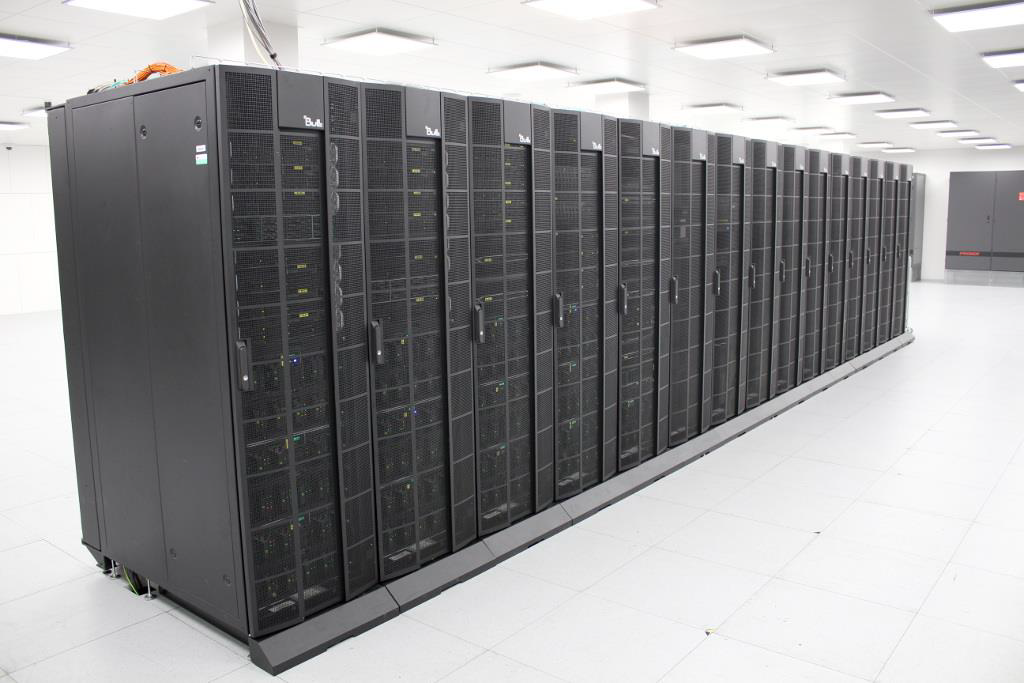
\includegraphics[width=0.5\textwidth]{anselm}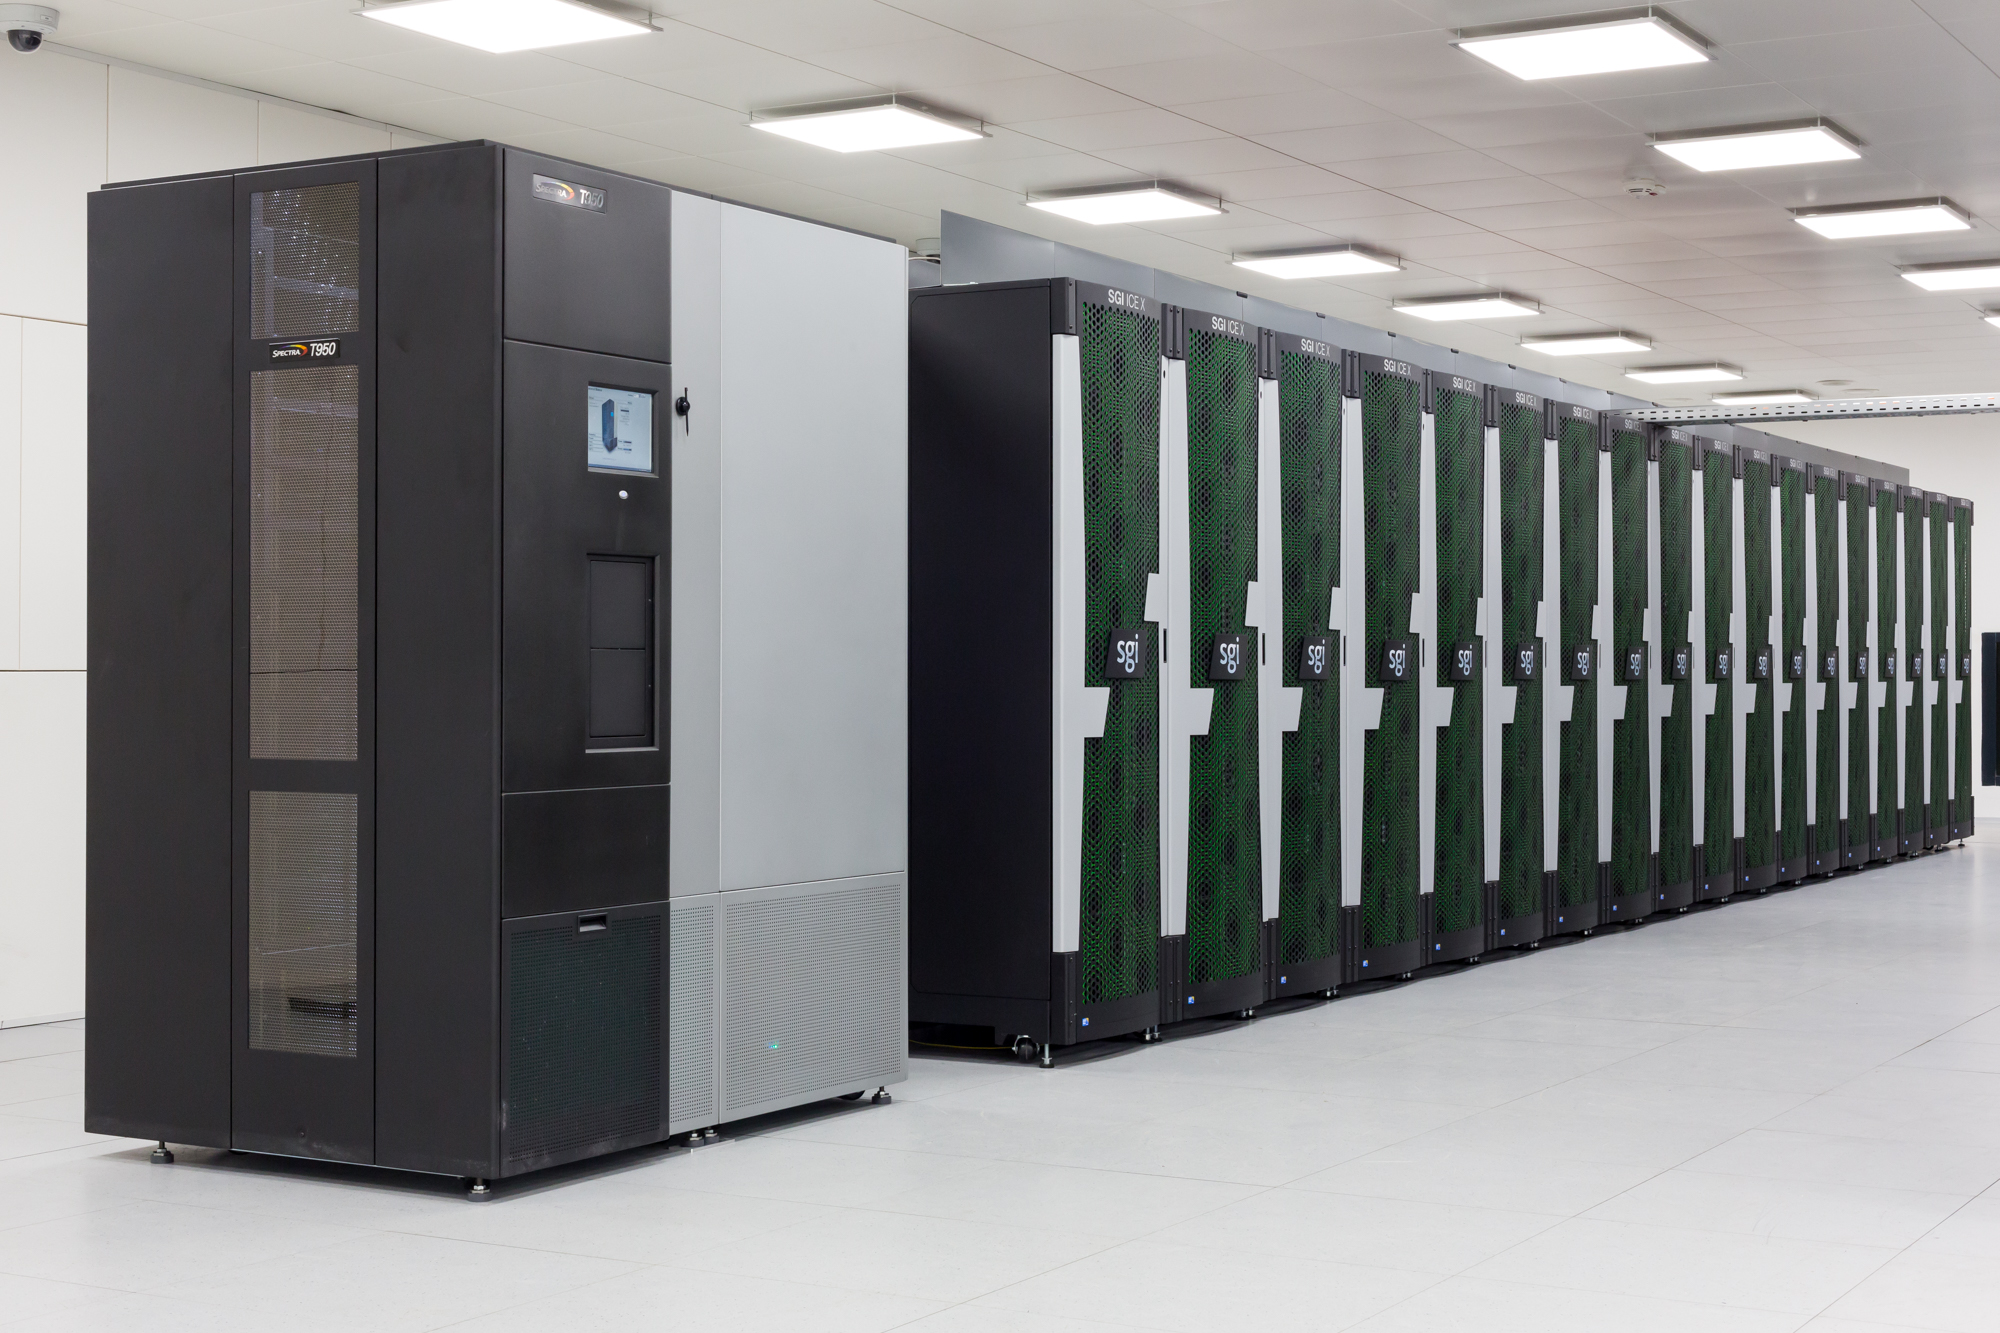
\includegraphics[width=0.5\textwidth]{salomon}

    \vspace{3mm}
    \centering \scriptsize Foto: Jaroslav Ožana, IT4Innovations
\end{frame}

\begin{frame}{Execution stack}
	\centering \animation[0.13]{development-pipeline}{4}
\end{frame}

\begin{frame}[fragile]{How do you get performance?}
	% algorithm
	% BTW: yes, this monster does compile, to a single instruction at -O3
	% (I have no idea what type is range)
	\begin{overprint}
		\onslide<2>
		\Large Language?
		\begin{tcolorbox}
		\begin{minted}[fontsize=\scriptsize,tabsize=2]{cpp}
template <class L, class R>
constexpr auto add_two_numbers(const std::tuple<L, R>& numbers) {
	static_assert(std::is_copy_constructible<decltype(
		std::get<0>(numbers) + std::get<1>(numbers))>::value);

	// use a lambda so it gets inlined
	return [&numbers](const auto& tup) {
		auto [x, y] = tup;
		auto range = {x, y};
		return std::accumulate(std::begin(range), std::end(range), 0);
	}(numbers);
}
		\end{minted}
		\end{tcolorbox}
	\end{overprint}
\end{frame}
\begin{frame}[fragile]{How do you get performance?}
	% inlining, compiler optimizations
	% -O5
	\Large Compiler?
	\begin{minted}[fontsize=\normalsize]{bash}
g++ -O5 -fludicrous-math -pthread-please-scale code.cpp
	\end{minted}
\end{frame}
\begin{frame}{How do you get performance?}
	% Frontend - fetches, decodes, uops
	% Backend - schedules into execution ports, writes to memory
	\Large Hardware?

	\vspace{1mm}
	\animation[1]{haswell-diagram}{3}
\end{frame}
\begin{frame}{How do you get performance?}
	\Large
	\begin{itemize}
		\item<1-> Use the right algorithm
		\item<2-> Implement and compile it properly
		\item<3-> \only<3>{Tune it to the underlying architecture}\textbf{\only<4>{Tune it to the underlying architecture}}
	\end{itemize}
\end{frame}
\begin{frame}{Software vs hardware complexity}
	\Large
	\begin{itemize}
		\item[] \texttt{C++} 17 final draft: \uncover<2->{1622 pages}

		\vspace{3mm}
		\item<3->[] Intel x64 manual:\ \ \uncover<4->{\textbf{4846} pages!}
	\end{itemize}
	\only<2->{\footnotetext[1]{\tiny{http://www.open-std.org/jtc1/sc22/wg21/docs/papers/2017/n4659.pdf}}}
	\only<4>{\footnotetext[2]{\tiny{https://software.intel.com/sites/default/files/managed/39/c5/325462-sdm-vol-1-2abcd-3abcd.pdf}}}
\end{frame}
\begin{frame}{CPU demonstration snippet found online}
	\begin{tcolorbox}
		\centering 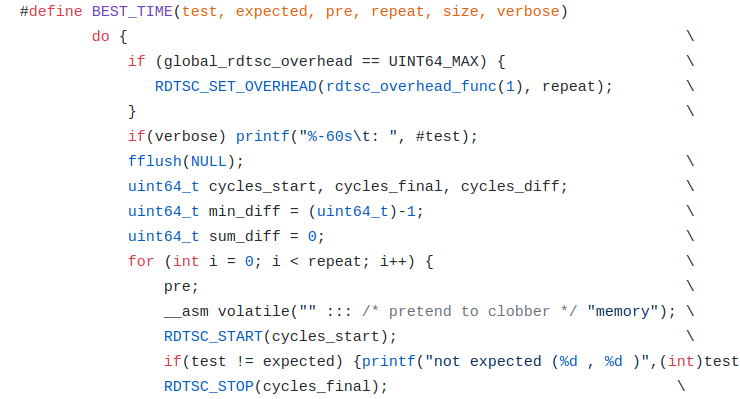
\includegraphics[width=0.9\textwidth]{lemire_short_tp}
	\end{tcolorbox}
\end{frame}

\begin{frame}{Hardware effects}
	% invited here to talk about this
	\begin{center}{\large \url{https://github.com/kobzol/hardware-effects}}

	\vspace{3mm}
	Demonstrations of CPU design ramifications\end{center}

	\begin{itemize}
		\item<2-> Short, comprehensible \texttt{C++} programs
		\item<3> \texttt{-O3} 
	\end{itemize}
\end{frame}

\begin{frame}
	\begin{center}\Huge Let's see some examples\end{center}
\end{frame}
\begin{frame}{Most upvoted Stack Overflow question}
	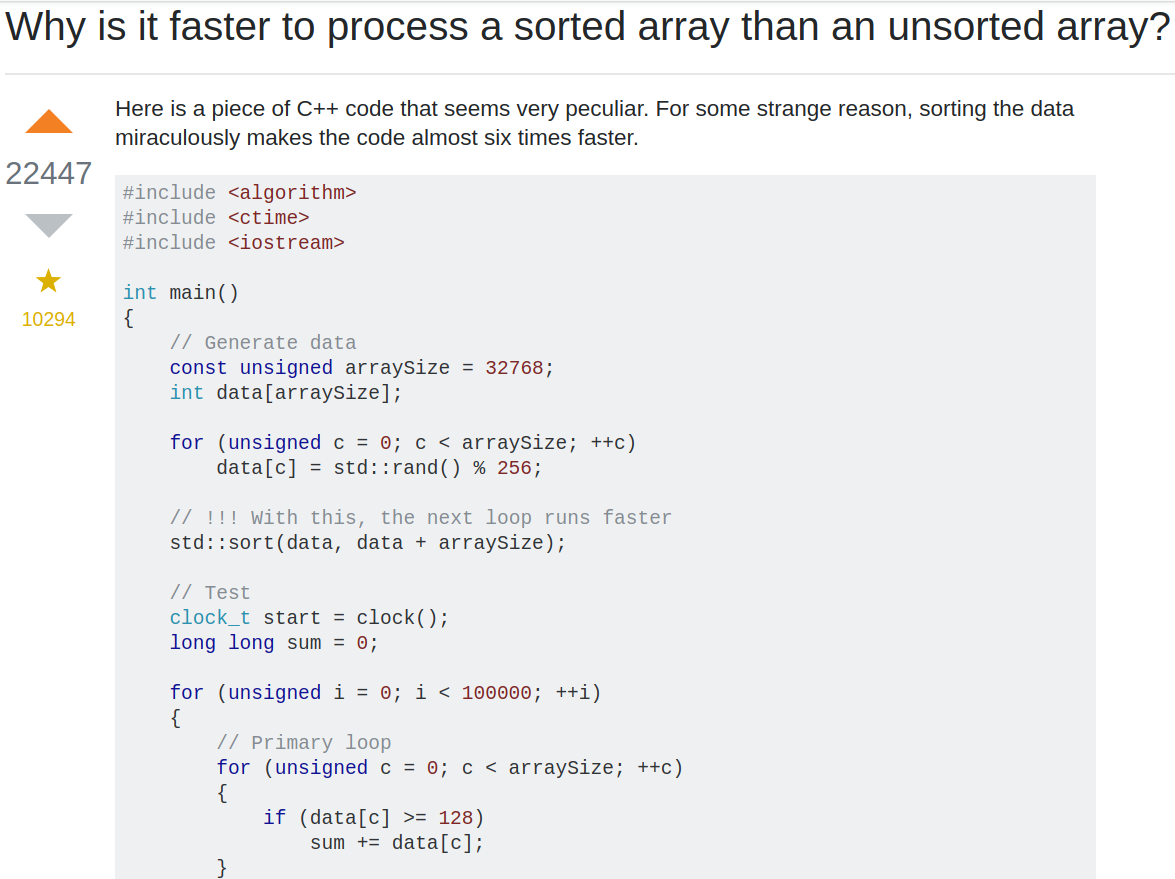
\includegraphics[width=\textwidth]{stack-overflow}
\end{frame}
\begin{frame}{Profiling tools - Intel Amplifier (VTune)}
	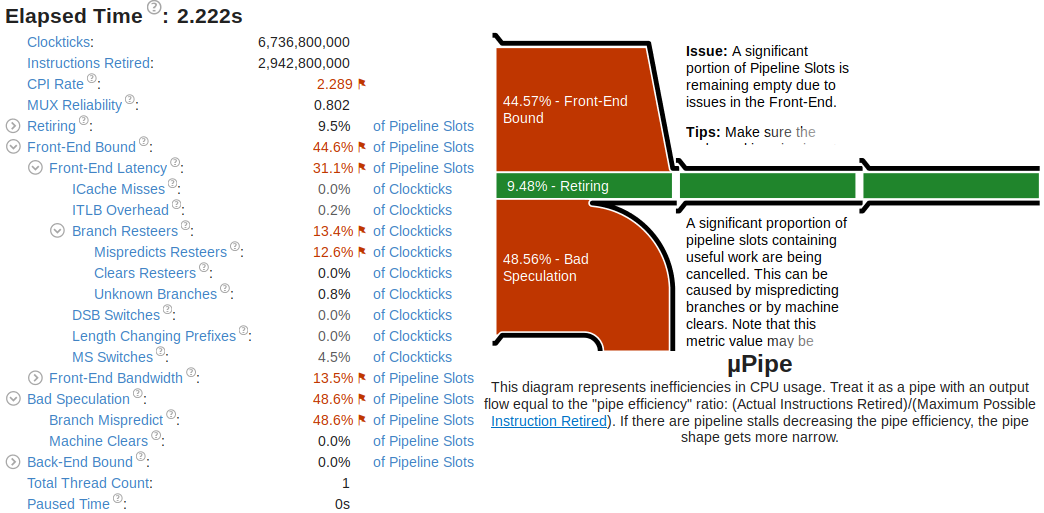
\includegraphics[width=\textwidth]{vtune}
\end{frame}
\begin{frame}[fragile]{Profiling tools - perf}
	\begin{tcolorbox}
	\begin{minted}[style=perldoc]{bash}
$ perf stat ./my-program

	          948  task-clock (msec)
	          197  page-faults
	3 254 047 397  cycles
	1 483 156 512  instructions
	  421 718 831  branches
	  102 931 445  branch-misses

$ perf list # lists all available counters
	  \end{minted}
	  \end{tcolorbox}
\end{frame}
\begin{frame}{CPU pipeline 101}
	\animation{pipeline}{6}
\end{frame}
\begin{frame}{CPU pipeline 101}
	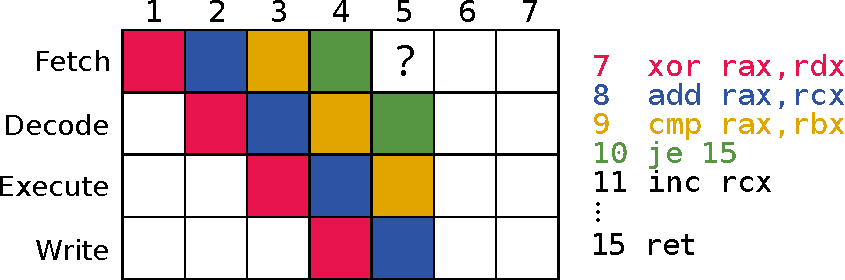
\includegraphics[width=\textwidth]{pipeline6}

	\vspace{5mm}
	\centering \large The CPU predicts the result of conditional branches

	\vspace{3mm}
	\uncover<2>{Misprediction costs \textapprox15-20 cycles!}
\end{frame}
\begin{frame}{Branch predictor}
	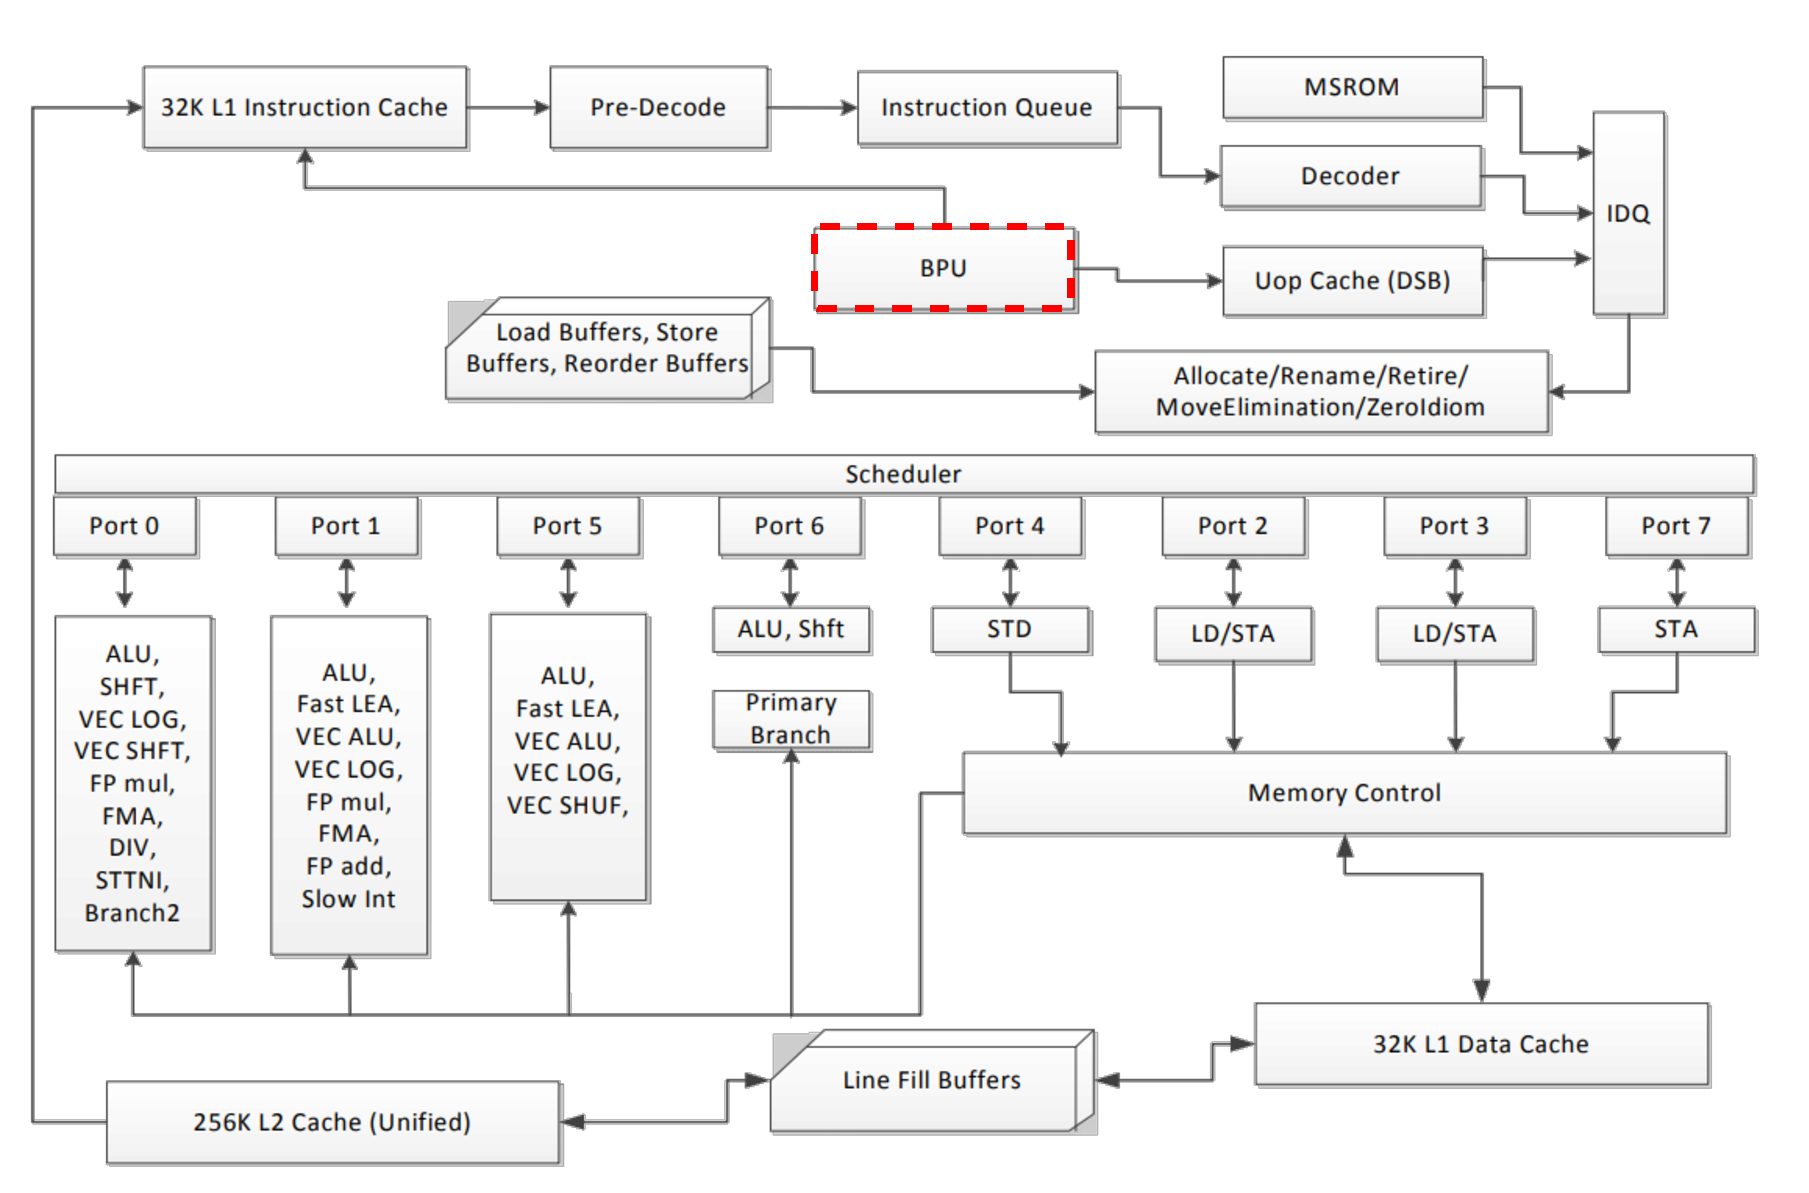
\includegraphics[width=\textwidth]{haswell-diagram4}
\end{frame}
\begin{frame}{Branch prediction - random array}
	\animation{branch-predictor}{7}
\end{frame}
\begin{frame}{Branch prediction - sorted array}
	\animation{branch-predictor-sorted}{7}
\end{frame}
\begin{frame}[fragile]{How to help the branch predictor?}
	\begin{itemize}
		\item More predictable data
		\item<2-> Compiler hints
		\begin{tcolorbox}
		\begin{minted}{cpp}
if (__builtin_expect(will_it_blend(), 1)) {
	// this branch is likely to be taken
}
		\end{minted}
		\end{tcolorbox}
		\begin{itemize}
			\item<3-> Automated with Profile-guided optimization (PGO)
		\end{itemize}
		\item<4> Remove branches
	\end{itemize}
\end{frame}
%\begin{frame}[fragile]{How to remove branches?}
%		This branch:
%		\begin{tcolorbox}
%		\begin{minted}{cpp}
%if (x < 6) {
%	sum += x;
%}
%		\end{minted}
%		\end{tcolorbox}
%		\uncover<2->{Could be rewritten as:}
%		\begin{itemize}
%			\item<2-> \texttt{sum += x * (x < 6);}
%			\item<3-> \texttt{sum += \textapprox((5 - x) >{}> 31) \& x;}
%		\end{itemize}
%		
%		\vspace{3mm}
%		\uncover<4>{Dedicated support in x86 hardware: \texttt{CMOV}}
%\end{frame}
\begin{frame}{Indirect jumps}
	Target of the jump is unknown at compile/link time
	\begin{itemize}
		\item<2-> Function pointers
		\item<3-> Function return addresses
		\item<4> Virtual methods
	\end{itemize}
\end{frame}
\begin{frame}{Virtual method overhead}
	\begin{itemize}
		\item Increased object size
			\begin{itemize}
				\item More data cache misses
			\end{itemize}
		\item<2-> Extra indirection
		\item<3-> Prevents inlining
		\item<4-> Branch target mispredictions
			\begin{itemize}
				\item<5> Branch target predictor
			\end{itemize}
	\end{itemize}
\end{frame}
\begin{frame}[fragile, t]{How to measure it?}
	\begin{center}
		{\Large \texttt{branch-misses}}

		How many times CPU mispredicted a branch or an indirect jump?
	\end{center}

	\vspace{8mm}
	\begin{tcolorbox}
	\begin{minted}[style=perldoc]{bash}
$ perf stat -e branch-misses ./my-program

	72 480 534 branch-misses
	\end{minted}
	\end{tcolorbox}
\end{frame}
\begin{frame}{False sharing}
	\animation{false-sharing-array}{6}
\end{frame}
\begin{frame}{False sharing}
	\begin{itemize}
		\item Multiple threads access the same cache line at the same time
		\item<2-> At least one of them writes to it
	\end{itemize}
\end{frame}
\begin{frame}{False sharing}
	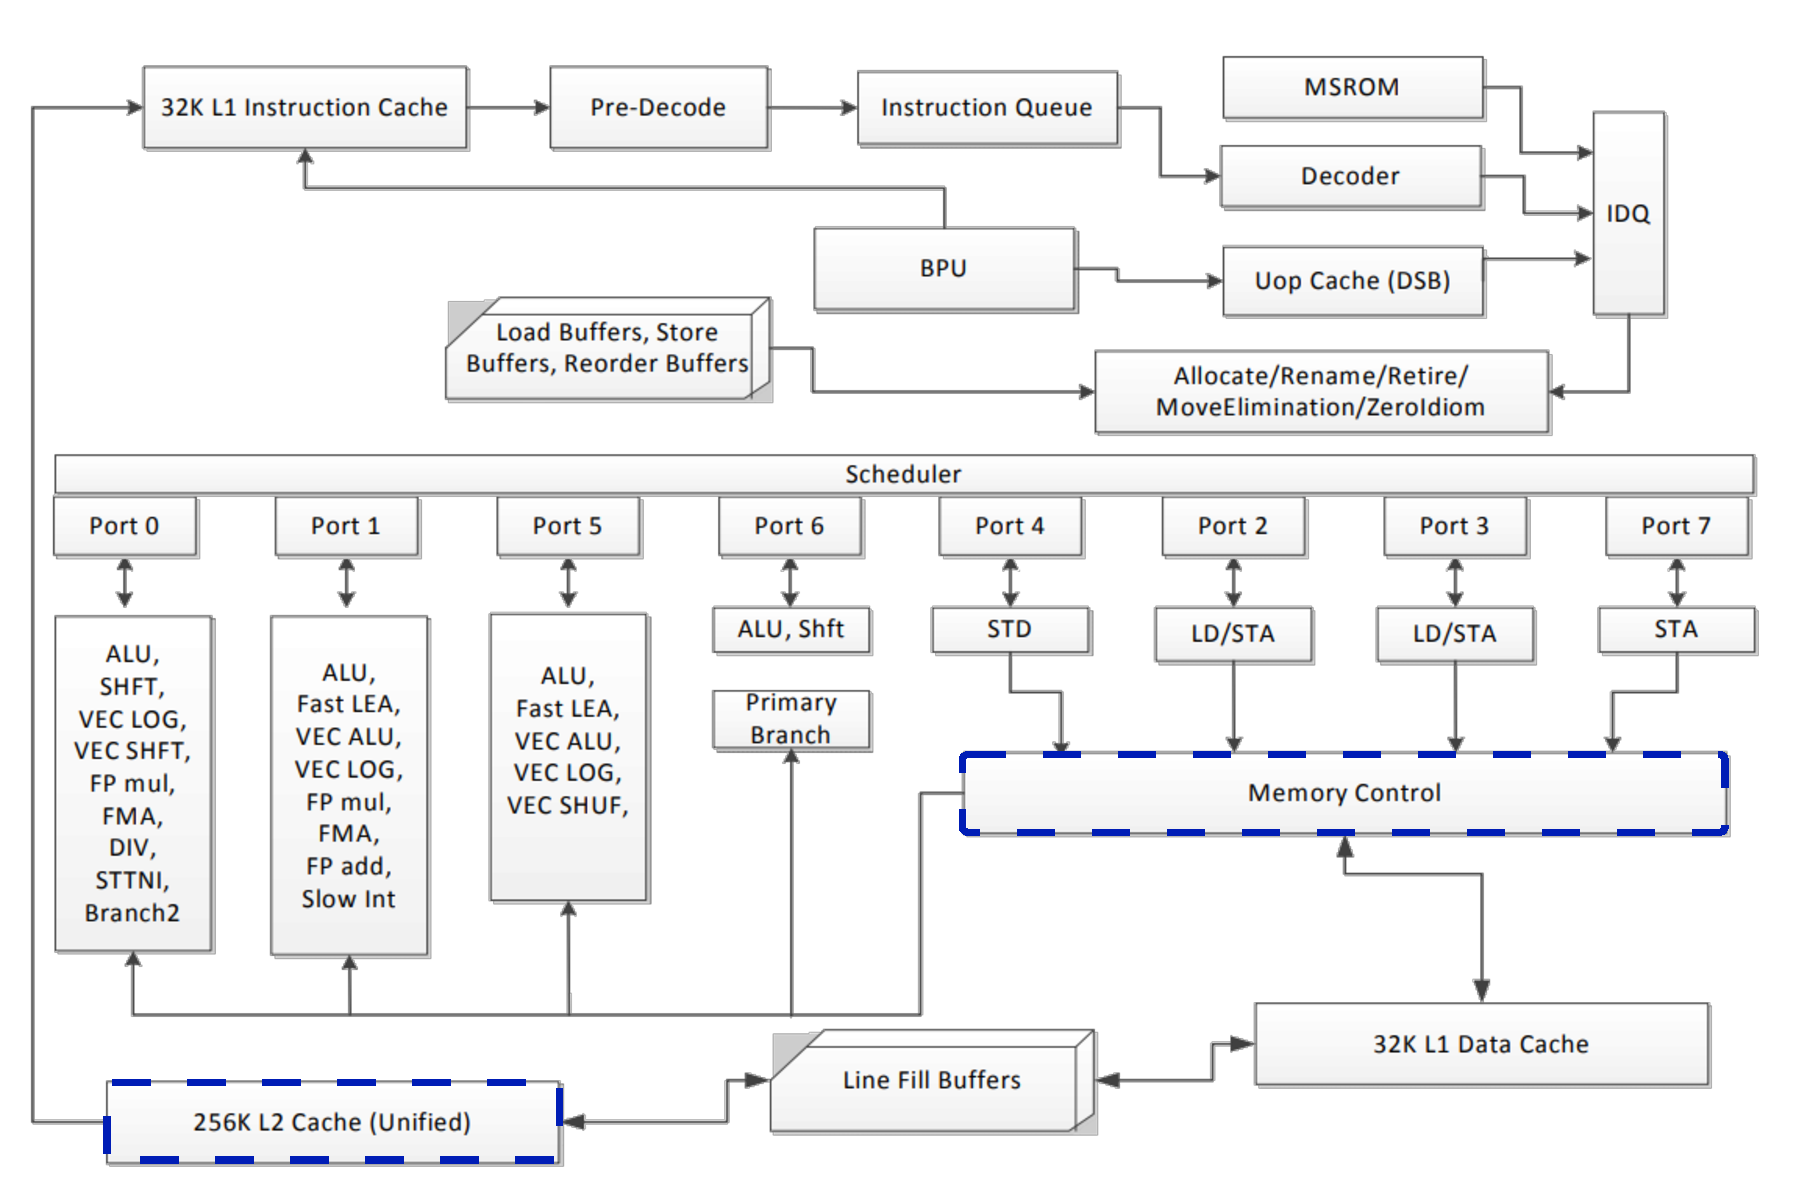
\includegraphics[width=\textwidth]{haswell-diagram5}
\end{frame}
\begin{frame}{False sharing}
	\animation{false-sharing}{9}
\end{frame}
\begin{frame}[fragile, t]{How to measure it?}
	\begin{center}
		{\Large \texttt{l2\_rqsts.all\_rfo}}
	
		How many times some core invalidated data in other cores?
	\end{center}

	\vspace{8mm}
	\begin{tcolorbox}
	\begin{minted}[style=perldoc]{bash}
$ perf stat -e l2_rqsts.all_rfo ./my-program

	90 324 547 l2_rqsts.all_rfo
	\end{minted}
	\end{tcolorbox}
\end{frame}
\begin{frame}[fragile]{How to fix it?}
	\only<1>{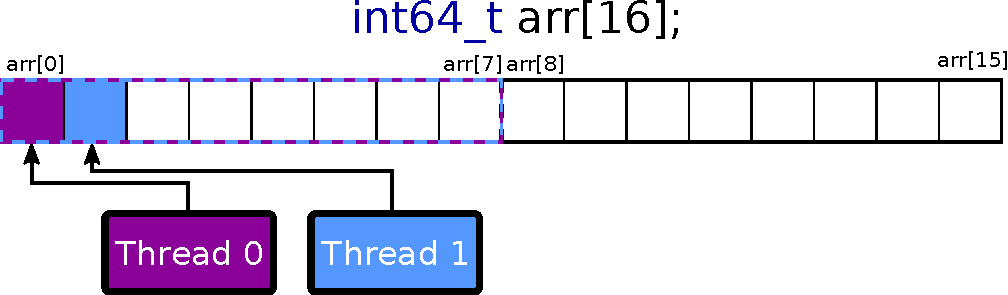
\includegraphics[width=\textwidth]{false-sharing-array6.pdf}}
	\only<2>{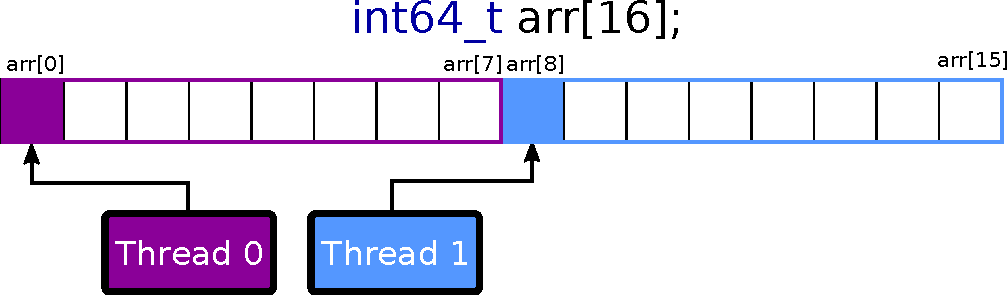
\includegraphics[width=\textwidth]{false-sharing-array7.pdf}}
\end{frame}
\begin{frame}{Denormal FP numbers}
	Numbers with zero exponent and non-zero significand

	\vspace{3mm}
	\uncover<2->{\fphalf{0000000000000001}
	$(-1)^{\textcolor{purple}{0}} * 2^{\textcolor{darkgreen}{00000} - \textbf{01110}} * \textbf{0}.\textcolor{lightblue}{0000000001}$}
	\begin{itemize}
		\item<2-> Numbers close to zero
		\item<3-> Hidden bit 0, smaller bias
	\end{itemize}

	\uncover<4>{\begin{center}\Large Operations on denormal numbers are slow!\end{center}}
\end{frame}
\begin{frame}{Denormal FP numbers}
	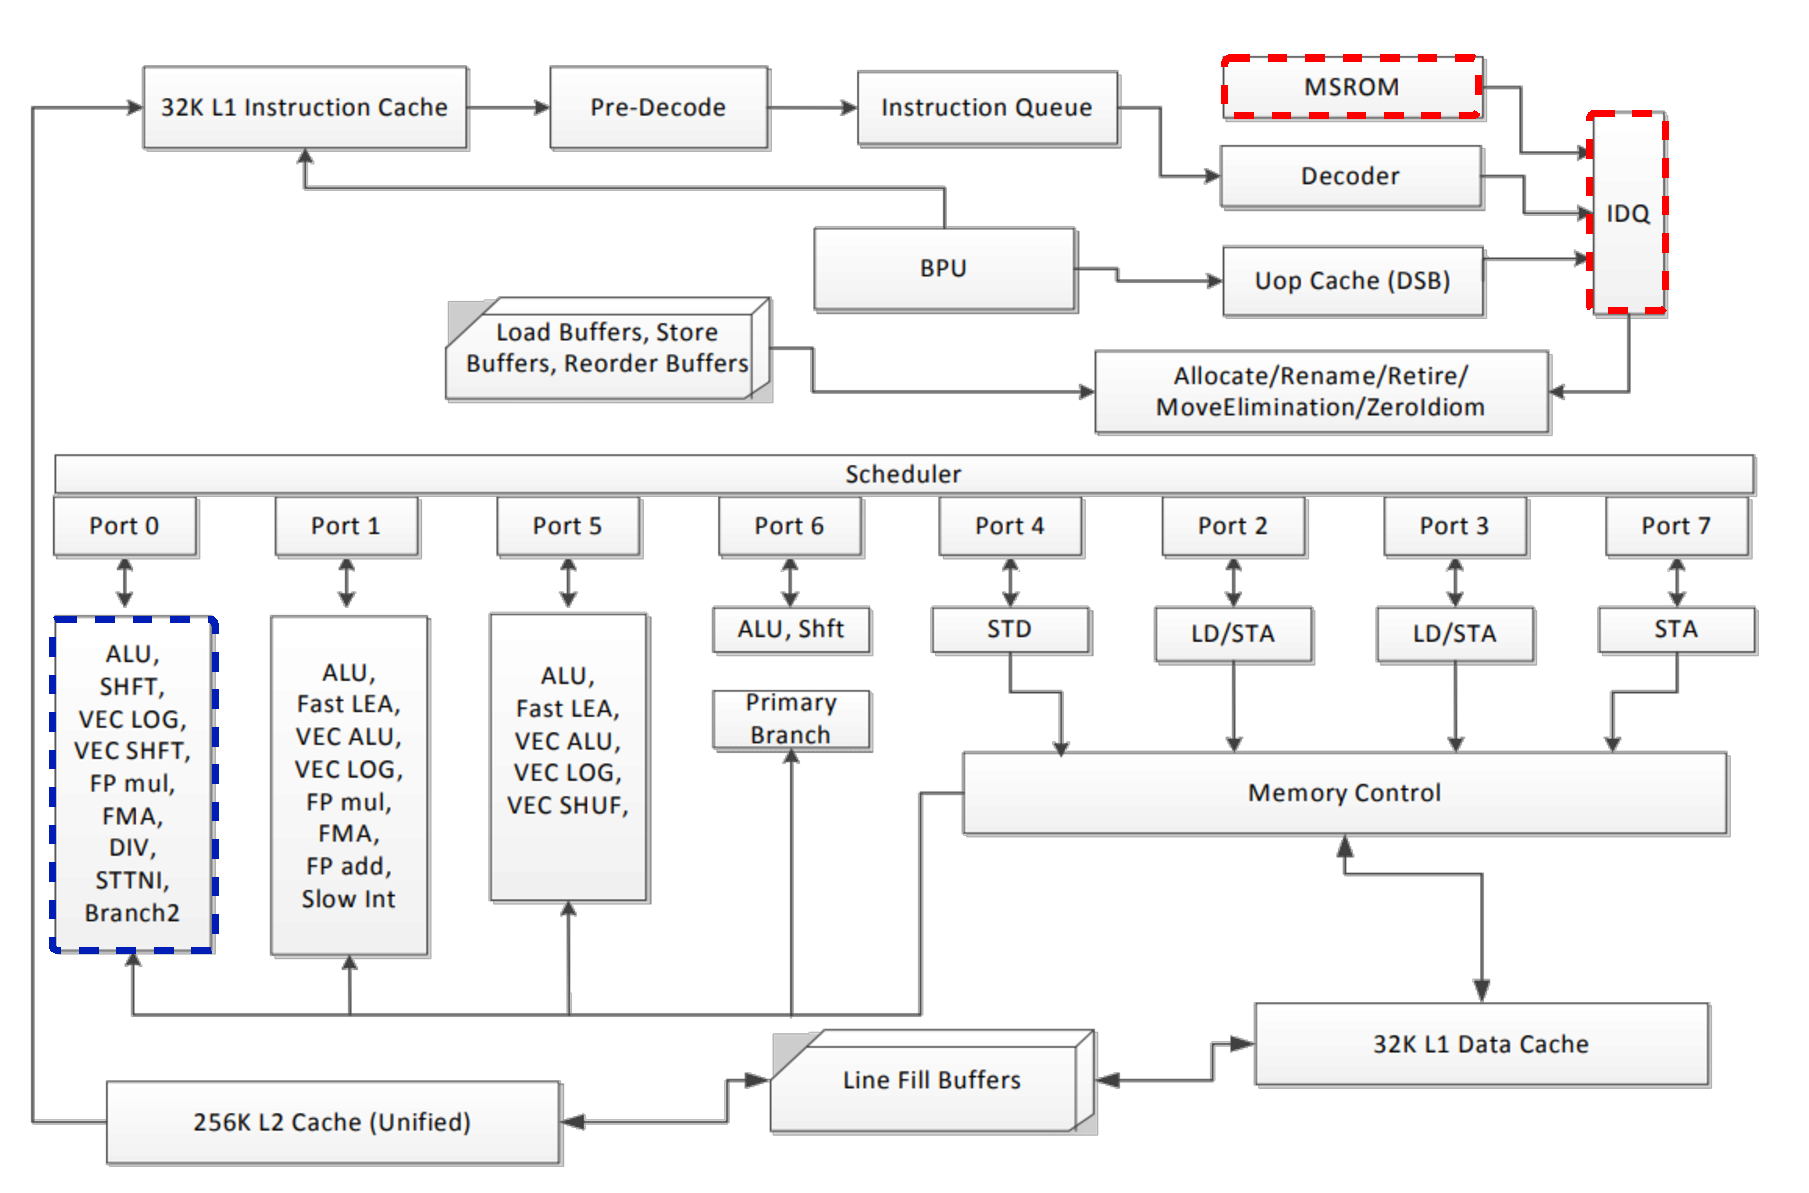
\includegraphics[width=\textwidth]{haswell-diagram6}
\end{frame}
\begin{frame}[fragile, t]{How to measure it?}
	\begin{center}
		{\Large \texttt{fp\_assist.any}}

		How many times the CPU switched to the microcode FP handler?
	\end{center}

	\begin{tcolorbox}
	\begin{minted}[style=perldoc]{bash}
$ perf stat -e fp_assist.any ./my-program

	9 437 184 fp_assist.any
	\end{minted}
	\end{tcolorbox}
\end{frame}
\begin{frame}[fragile]{How to fix it?}
	\begin{itemize}
		\item Compiler switch \texttt{-ffast-math}
		\item<2-> Set CPU flags:
			\begin{itemize}
				\item Flush-to-zero - treat denormal outputs as 0
				\item Denormals-as-zero - treat denormal inputs as 0
			\end{itemize}

			\vspace{5mm}
			\begin{overprint}
				\onslide<3>
				\begin{tcolorbox}
				\begin{minted}{cpp}
_mm_setcsr(_mm_getcsr() | 0x8040);
				\end{minted}
				\end{tcolorbox}

				\onslide<4>
				\begin{tcolorbox}
				\begin{minted}[fontsize=\footnotesize]{cpp}
_MM_SET_FLUSH_ZERO_MODE(_MM_FLUSH_ZERO_ON);
_MM_SET_DENORMALS_ZERO_MODE(_MM_DENORMALS_ZERO_ON);
				\end{minted}
				\end{tcolorbox}
			\end{overprint}
	\end{itemize}
\end{frame}

\begin{frame}{There are loads of other effects}
	\begin{itemize}
		\item NUMA effects
		\item Data dependencies between instructions
		\item 4k aliasing
		\item Cache conflicts
		\item Misaligned accesses
		\item Software prefetching
		\item Non-temporal stores \& cache pollution
		\item Bandwidth saturation
		\item AVX/SSE transition penalty
		\item \ldots
	\end{itemize}
\end{frame}

\begin{frame}[t]{Thanks!}
	\begin{center}
		{\Huge Thank you :-)}

		\vspace{10mm}
		{\Large For more examples visit:}

		{\large \url{https://github.com/kobzol/hardware-effects}}
		
		\vspace{10mm}
		{\large Jakub Beránek}
	\end{center}
\end{frame}

\begin{frame}{Useful stuff}
	\begin{itemize}
		\item \url{wikichip.org}
		\item Agner Fog optimization manual
		\item Intel x64 developer manual
		\item Compiler explorer :-)
		\item Intel intrinsics guide
		\item SIMD Visualiser
	\end{itemize}
\end{frame}

\end{document}
